\documentclass[12pt]{article}

\usepackage{amsmath}
\usepackage[margin=1in]{geometry}
\usepackage{hyperref}
\usepackage{graphicx}
\graphicspath{{./images/}}
\linespread{2}

\usepackage{pythontex}
\newcommand{\ohsheader}[3]{ #1 \par
    #2 \par %class
    \today \par
    #3 %assignment
}

\title{An Analysis of Visual Subitization Across Different Modes of Peripheral Vision}

\author{Juni Kim \\
Stanford Online High School}

\date{\today}

\begin{document} 

\maketitle

Subitization is the almost instantaneous ability of humans to visually deduce
the quantity of a certain object (or category) given that the number is small
enough. For numbers beyond four, humans will instinctually use a system of
counting and approximation that is less accurate and more time-consuming. When
one uses this process of subitizing, they are able to count objects with
minimal effort, as if it were an alternate form of perception. The study that
I conducted thus tries to test the effect that visual perception has on the
ability of one to subitize correctly.

Peripheral vision is the ability of humans to see objects that are not exactly
on the focus of the eye and are thus allocated less cognitive resources to
process. Testing the effect of peripheral vision on one's ability to subitize
would further unveil whether or not visual perception has a significant effect
on this ability.

Within my final project for OMSB9, I collected and analyzed data concerning the
ability of people to accurately count the number of objects in a drawing along
different angles of peripheral vision and the time in which an image was
flashed. I intend to find the accuracy of subitizing across different modes of
peripheral vision and as to the effect that reaction time has on accuracy.

\section{Methodology}

\subsection{Samples}
A sample of 5 people was used in this experiment (due to the lack of reachable
people as a result of COVID-19). I conducted tests on 4 different times (250ms,
500ms, 750ms, and 1000ms) and 3 different angles relative to straight ahead
($0^{\circ}$, $30^{\circ}$, $60^{\circ}$), leading to a net 12 different
variations on the test to perform. Each of these variations was done five times
per participant.

\subsection{Scripts}

In order to make the testing procedure more efficient, I wrote a set of PHP
scripts that could be run in a localhost setting and allow me to both run and record the
tests. The source code can be found in
\url{https://github.com/junikimm717/OMSB9-Final-Project/tree/main/website}.

\subsubsection{Testing Page}
The testing page is located in the /testing.php file.

Within the testing page, one may modify the GET parameters (which include the
participant name, angle being tested, and the time being tested) to conduct
different tests. When one clicks the ``conduct test" button, a randomly selected
picture (consisting of a certain number of clearly visible dots) will appear
for a duration of time equal to the one that was put in the GET parameters. The
participant was asked how many dots they believe (to their best guesses) were
in the picture that was flashed, and this is recorded. Once this test is
complete, the ``submit" button is clicked.

\subsubsection{Handler Page}
The handler is located in the /handler.php file.

The handler page records all of the data gained from the test through a POST
request (so that a particularly adept participant cannot simply scan the GET
parameters and evaluate their previous answers) and appends this data
into a file called data.txt (note that the file never gets overwritten).

The handler page also contains a pre-filled HTML form which you may
modify if you would like to change the settings for the next test.

\subsection{Physical Setup}
A sheet of 11x17 paper was used to make demarcations of 0, 30, and 60 degree
deviations in order to consistently align the monitor correctly. At the 0
degree line, an object would be placed (preferably one that is relatively thin)
for the participant to focus their fovea on while the test is taking place.
The computer is then placed on one of the lines (for testing a particular
angle), and the test can be run.


\begin{figure}
\centering
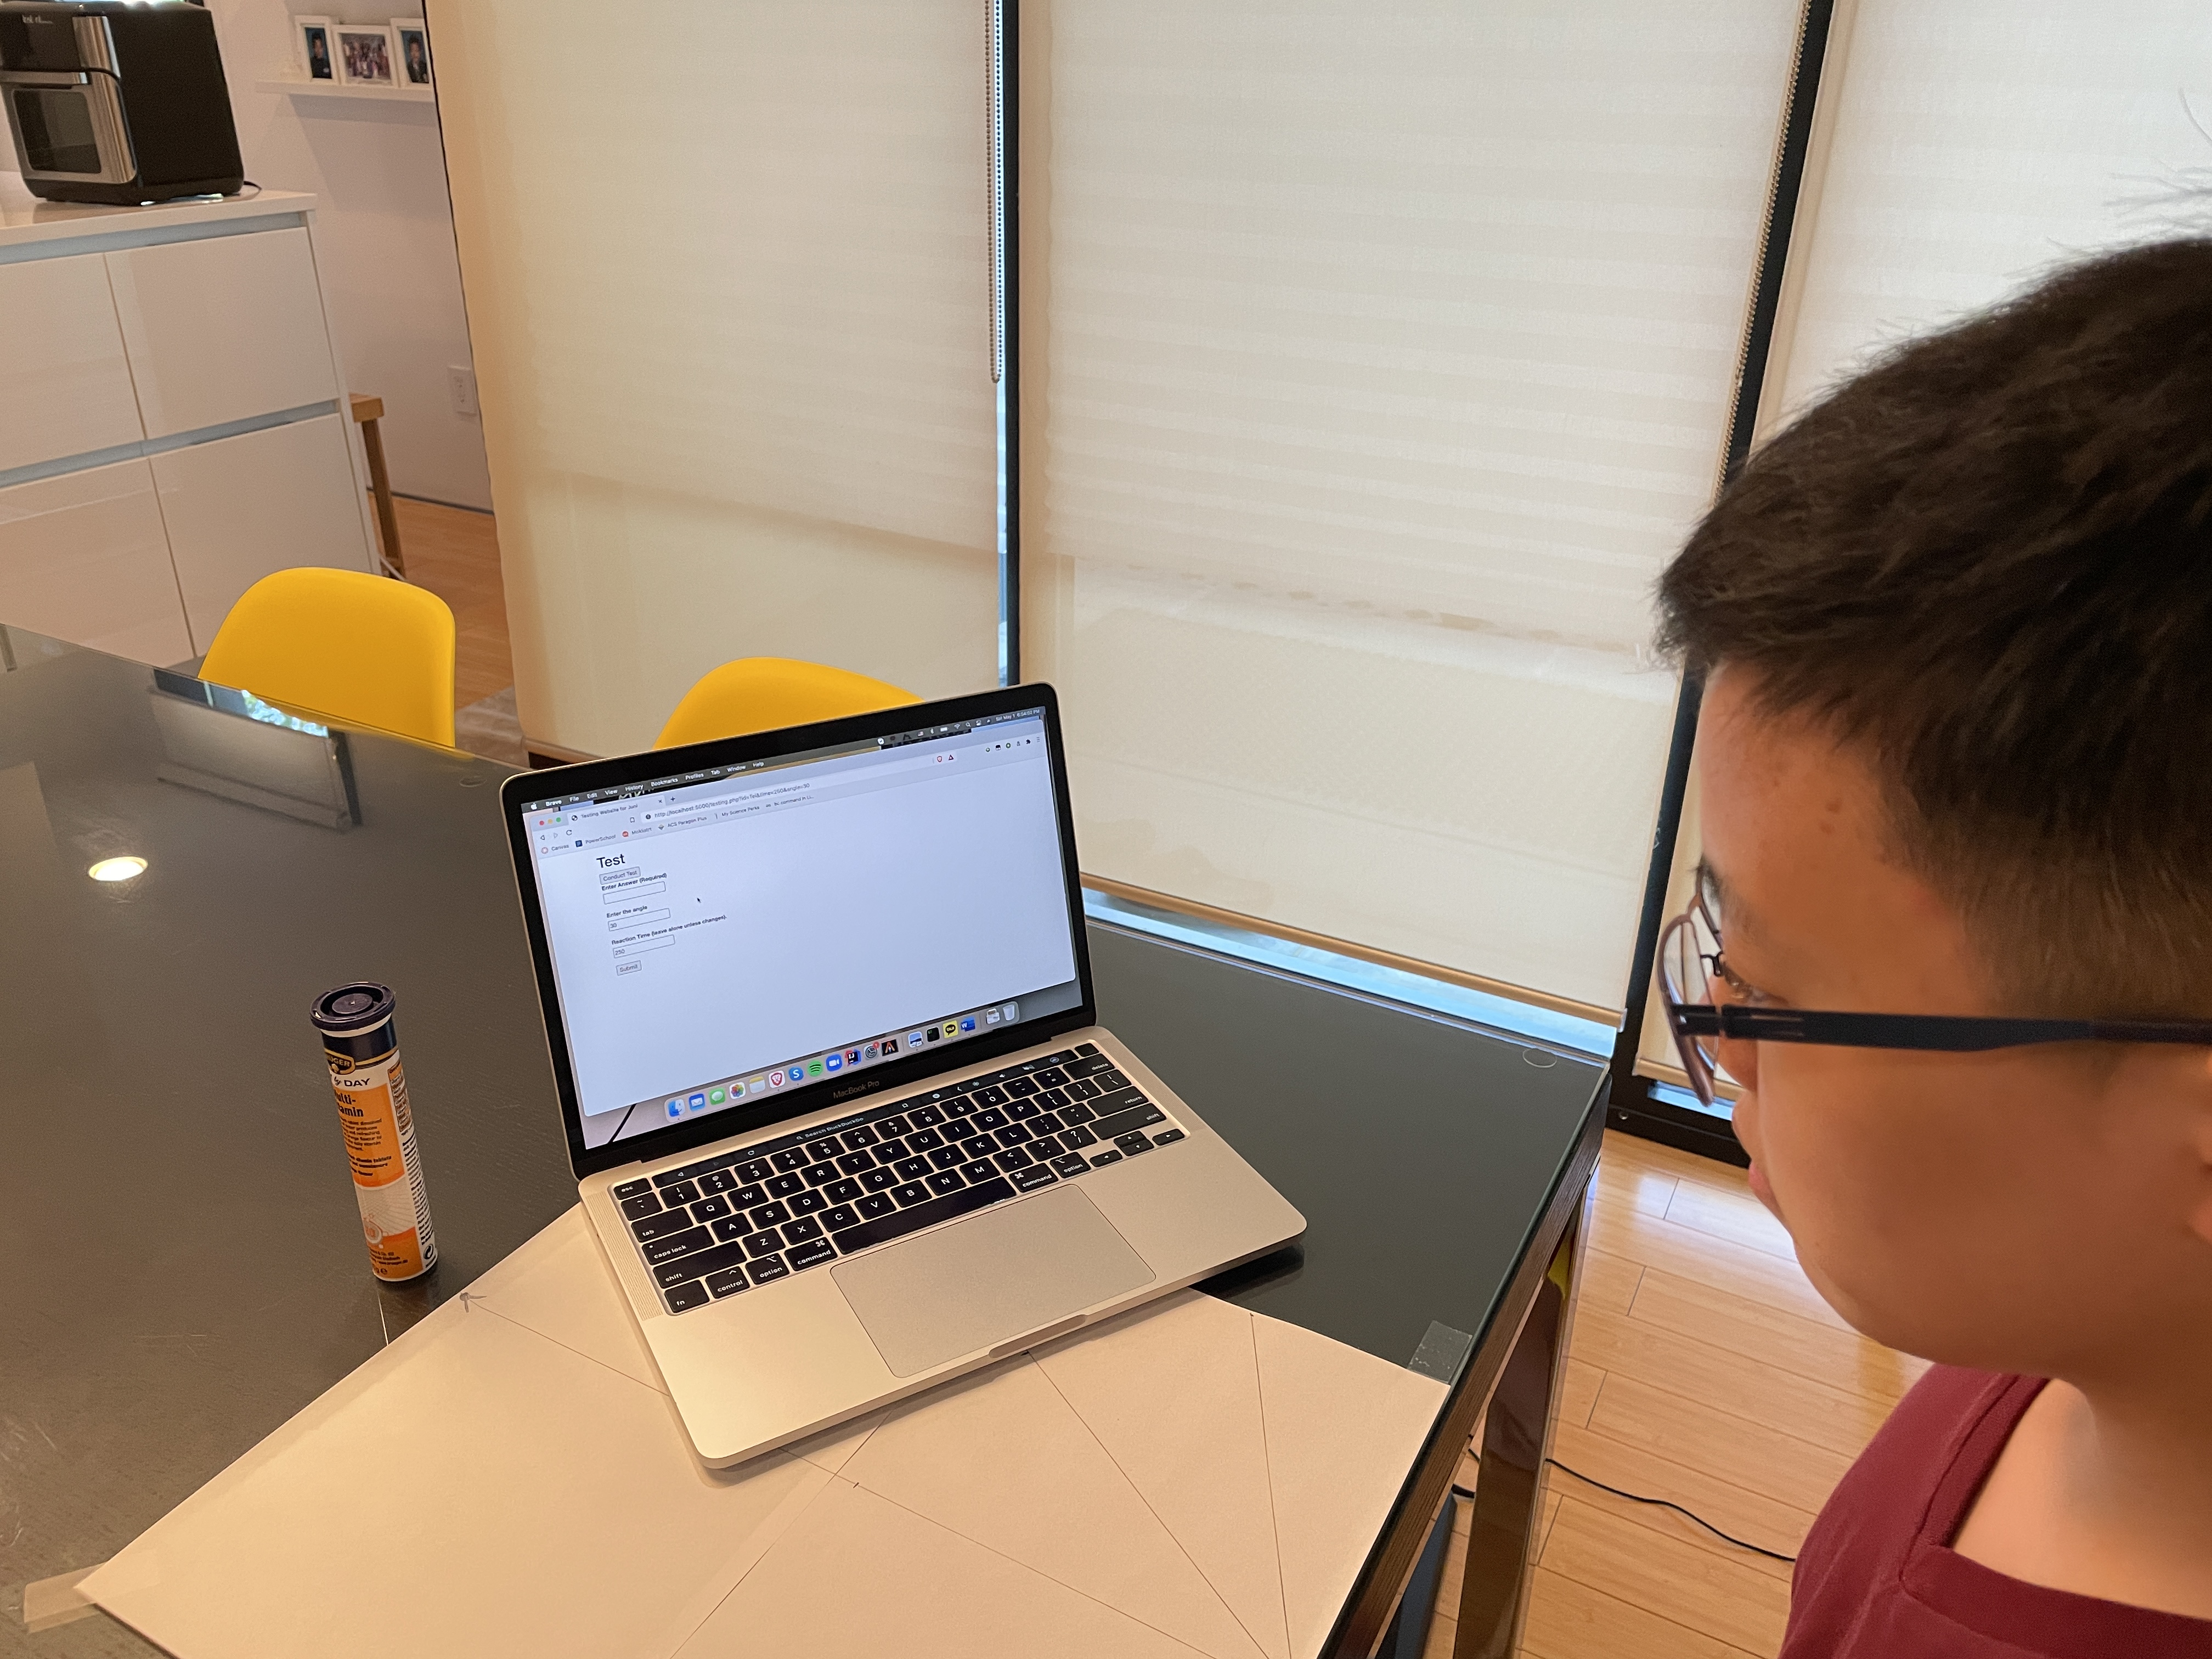
\includegraphics[scale=0.3]{diagram.JPG}
\caption{How the experiment should appear}
\end{figure}

\section{Data}
The raw (unprocessed) data can be found at \\
\url{https://github.com/junikimm717/OMSB9-Final-Project/tree/main/data/data.txt}
The data points seen below were all generated with matplotlib.

\begin{figure} [h]
\centering
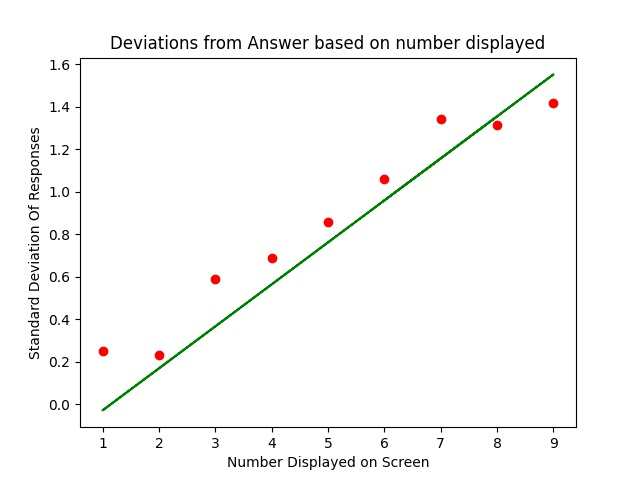
\includegraphics[scale=0.5]{regression.jpg}
\caption{Standard Deviation of Responses}
\end{figure}

\begin{figure} [h]
\centering
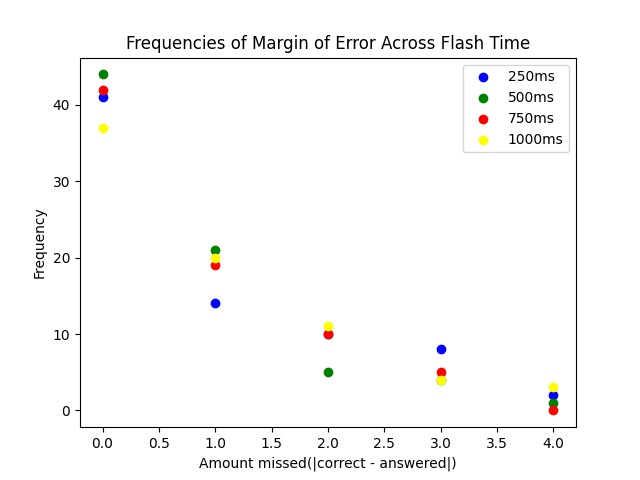
\includegraphics[scale=0.5]{reaction.jpg}
\caption{Accuracy across different times}
\end{figure}

\begin{figure} [h]
\centering
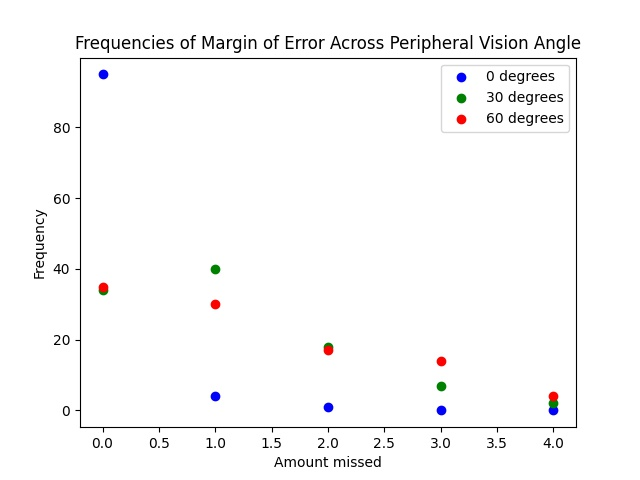
\includegraphics[scale=0.5]{angle.jpg}
\caption{Accuracy across different angles}
\end{figure}

\newpage
\section{Analysis}

Based on this raw data, I have been able to make some analyses and thus some
answers to my original questions going into the study.

\subsection{Deviations from answer}

For assessing the standard deviations of responses per answer, a linear
regression was plausible because there was minimal likelihood that the standard
deviation of responses would have a non-consistent distribution per response.

A PMCC test with the correct answer and the standard deviation of responses
exhibits a p-value of $2.1 \cdot 10^{-5}$ seems to indicate that there exists a
statistically highly significant positive correlation.

\subsection{Reaction Time and Error}

For assessing this correlation, I used a spearman rank correlation coefficient
(a non-parametric test) in order to assess if there was a significant monotonic
correlation between precision of the participant and the average reaction time.

The SRCC was equal to 0.027 and the p-value was 0.638, which indicates that,
with the data collected, there is no statistically significant
monotonic correlation between the time given for the participant to look at the
image and their precision.

\subsection{Accuracy based on Angle Viewed}

In order to assess whether or not participants were significantly more or less
accurate on at least one of the three angles at which they were tested, I
conducted a one-way ANOVA test (as the data is both parametric and has multiple samples).

The results show that $F=47.5$ and $p = 1.23 \cdot 10^{-18}$, which indicates
that there is a statistically highly significant difference between the results across
different angles.

\subsection{Near Peripheral Vision vs Far Peripheral Vision?}

In order to test whether or not near peripheral vision yielded a statistically
significantly better precision, I used a two-sample t-test.

The results indicated that $T = -1.707$ and $p = 0.121$, which indicates that
there is not a statistically significant difference between precision when
participants viewed the pictures from $30^{\circ}$ versus $60^{\circ}$.

\section{Conclusions}
Based on the statistically analyzed data, we have been able to prove that the
mean precision is different among tests from different angles of peripheral
vision, but we have been unable to prove such a difference exists between near
and far peripheral vision. As a benchmark, we have also shown a statistically
significant linear correlation between the amount of error within the
participants' tests and the number that was displayed in front of them, which
indicates (as others have previously shown), that the ability of subitization
decreases with time.

As I had constraints of time and accuracy as a result of being within the
COVID-19 pandemic, I was unable to get a larger set of peripheral vision angles
to check, which might have allowed me to do a correlation analysis and thus
gain better insights. Other studies might also be able to obtain more
volunteers than I have been able to.

\end{document}
